\chapter{Composición de velocidades, conos de luz y cuatro-vectores}

\section{Dos sistemas de referencia en una misma vía ferroviaria}

La transformación de Lorentz deducida anteriormente se refería a una geometría deliberadamente restringida: todo movimiento relativo tenía lugar a lo largo de un eje. Imaginemos una larga vía ferroviaria. Un grupo de observadores permanece en la estación; otro viaja en un tren que se desplaza por la vía. Las direcciones transversales están presentes, pero no intervienen hasta que se reincorporan más adelante.

Cada sistema de referencia es un sistema de coordenadas operativo. Las reglas métricas en reposo en ese sistema definen las coordenadas espaciales, y los relojes sincronizados en reposo en él definen el tiempo. El postulado que determina la relación entre ambos sistemas es que todos los observadores inerciales miden la misma velocidad de la luz.

La mayoría de los cálculos se hará con \(c=1\). El tiempo puede medirse en segundos y la distancia en segundos luz, o en años y años luz. Así, las velocidades se convierten en fracciones adimensionales de la velocidad de la luz. Cuando se necesiten unidades ordinarias, los factores de \(c\) se restituyen de manera única por consistencia dimensional; por ejemplo, \(v^2\) en un factor de Lorentz adimensional se convierte en \(v^2/c^2\).

\subsection{Transformaciones directa e inversa}

Supongamos que se produce un destello en algún punto del tren o cerca de él. Es un único suceso, independiente de quién lo describa. El observador de la estación le asigna \((x,t)\), mientras que el observador del tren le asigna \((x',t')\). En unidades \(c=1\),
\begin{align}
x'&=\gamma_v(x-vt),&
t'&=\gamma_v(t-vx),
\label{eq:sr2-direct}\\
\gamma_v&=\frac{1}{\sqrt{1-v^2}}.
\end{align}
Newton reconocería el desplazamiento \(x-vt\); el factor \(\gamma_v\) y la mezcla de \(x\) en \(t'\) son los cambios relativistas.

\begin{figure}[htbp]
\centering
\includegraphics[width=0.90\textwidth]{lecture_02_figure_01.png}
\caption{La transformación de Lorentz directa que relaciona las coordenadas de la estación \((x,t)\) con las del tren \((x',t')\).}
\lectureframe{00:07:52}
\end{figure}

La reciprocidad da la transformación inversa al cambiar el signo de la velocidad relativa:
\begin{align}
x&=\gamma_v(x'+vt'),&
t&=\gamma_v(t'+vx').
\label{eq:sr2-inverse}
\end{align}
La estación no está en reposo absoluto. Es simplemente el sistema de referencia que se denomina no primado, y el tren la ve moverse a \(-v\).

\begin{figure}[htbp]
\centering
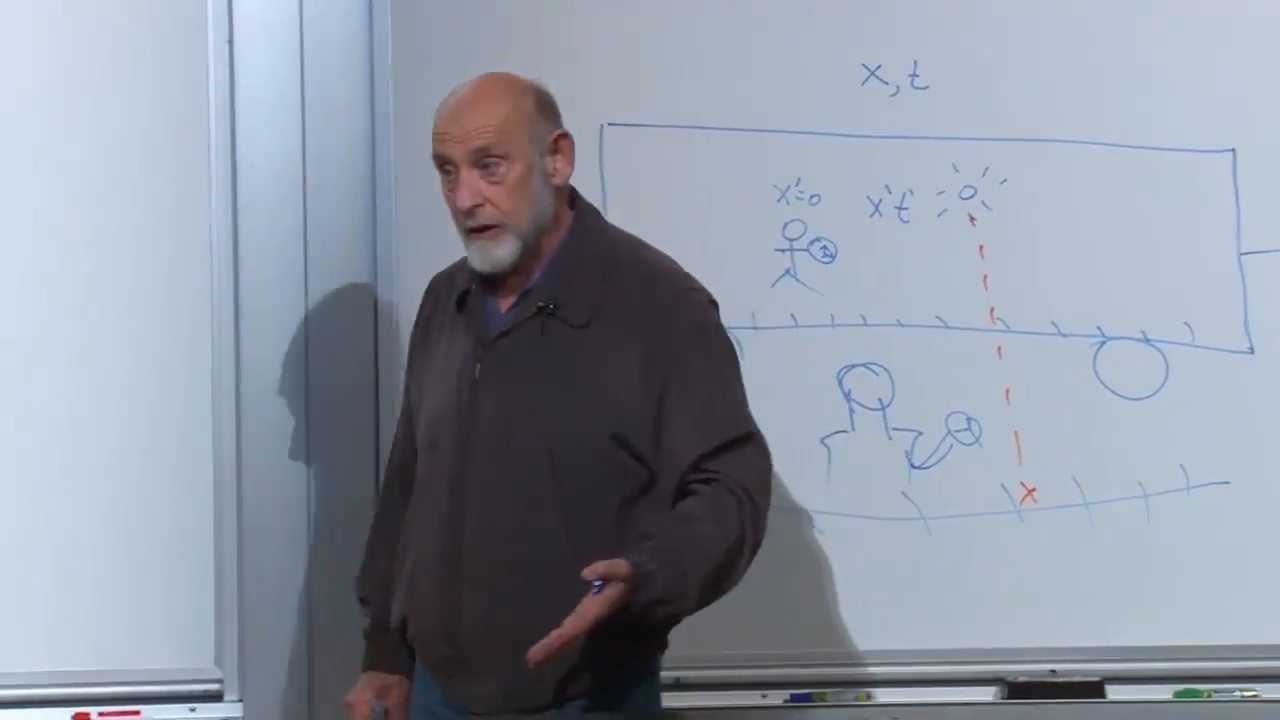
\includegraphics[width=0.90\textwidth]{lecture_02_figure_02.png}
\caption{La transformación inversa tiene el mismo factor de Lorentz y el signo opuesto de la velocidad relativa.}
\lectureframe{00:09:15}
\end{figure}

Para un impulso a lo largo de \(x\), las coordenadas transversales no cambian:
\begin{equation}
y'=y,
\qquad
z'=z.
\end{equation}

La velocidad relativa puede leerse de la ecuación espacial sin examinar su denominador. El origen del tren se define mediante \(x'=0\) y, por tanto,
\begin{equation}
x'=0
\quad\Longleftrightarrow\quad
x-vt=0
\quad\Longleftrightarrow\quad
x=vt.
\label{eq:sr2-origin-worldline}
\end{equation}
El coeficiente de \(t\) en esta línea de universo es la velocidad del tren en las coordenadas de la estación.

\section{Tres sistemas de referencia y composición de impulsos}

Coloquemos un cochecito dentro del tren. El tren se mueve a velocidad \(v\) respecto de la estación, mientras que el cochecito avanza por el pasillo a velocidad \(u\) respecto del pasajero del tren. Llamemos \(w\) a la velocidad del cochecito respecto de la estación. La intuición newtoniana sugiere \(w=u+v\), pero serán las transformaciones de Lorentz las que decidan.

Ahora hay tres sistemas de coordenadas:
\begin{equation}
(x,t),\qquad (x',t'),\qquad (x'',t'').
\end{equation}
El primero corresponde a la estación, el segundo al tren y el tercero al cochecito. Entre el tren y el cochecito,
\begin{align}
x''&=\gamma_u(x'-ut'),&
t''&=\gamma_u(t'-ux'),
\label{eq:sr2-second-boost}\\
\gamma_u&=\frac{1}{\sqrt{1-u^2}}.
\end{align}

\begin{figure}[htbp]
\centering
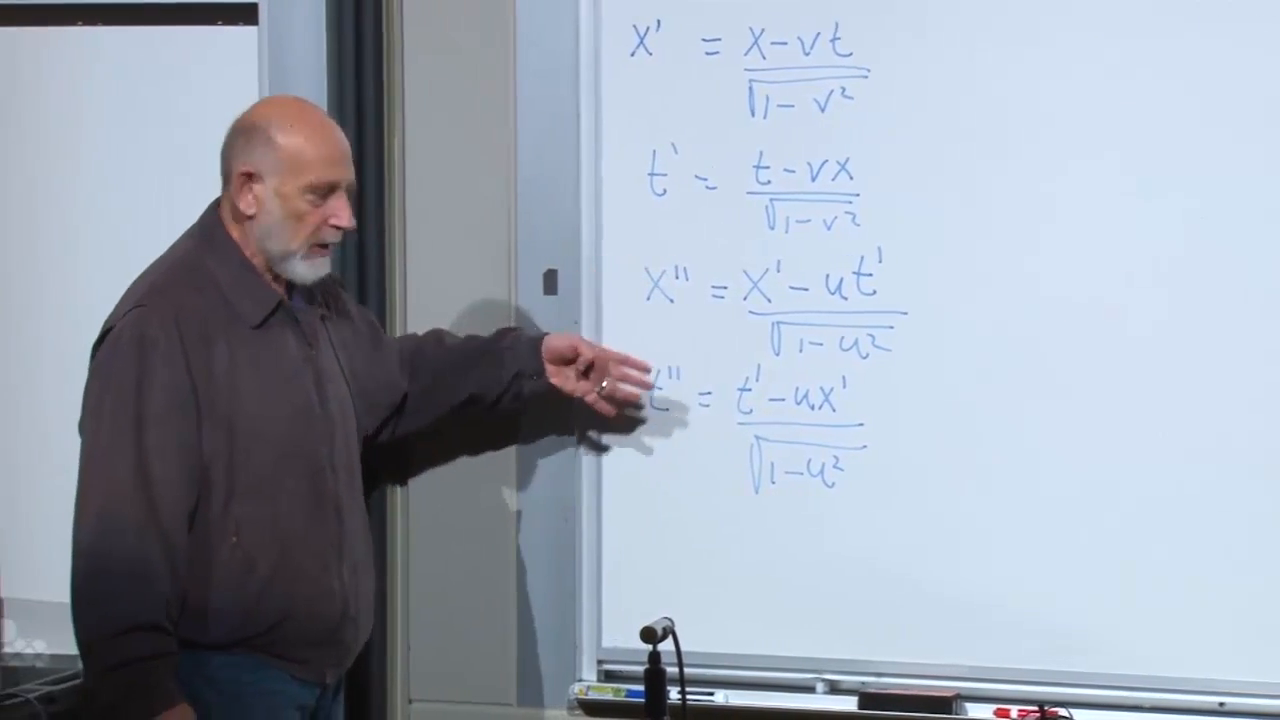
\includegraphics[width=0.90\textwidth]{lecture_02_figure_03.png}
\caption{A las fórmulas directas de la estación al tren les sigue una segunda transformación de Lorentz, de las coordenadas primas a las doblemente primas.}
\lectureframe{00:14:55}
\end{figure}

\subsection{Sustituir un impulso en el otro}

La ecuación espacial basta para hallar \(w\). Sustituyamos \eqref{eq:sr2-direct} en la primera ecuación de \eqref{eq:sr2-second-boost}:
\begin{align}
x''
&=\gamma_u(x'-ut')\\
&=\gamma_u\gamma_v\left[(x-vt)-u(t-vx)\right]\\
&=\gamma_u\gamma_v\left[(1+uv)x-(u+v)t\right].
\label{eq:sr2-composed-space}
\end{align}
Los dos signos menos del término \(uvx\) dan un signo positivo; los dos términos temporales se combinan como \(-(u+v)t\).

\begin{figure}[htbp]
\centering
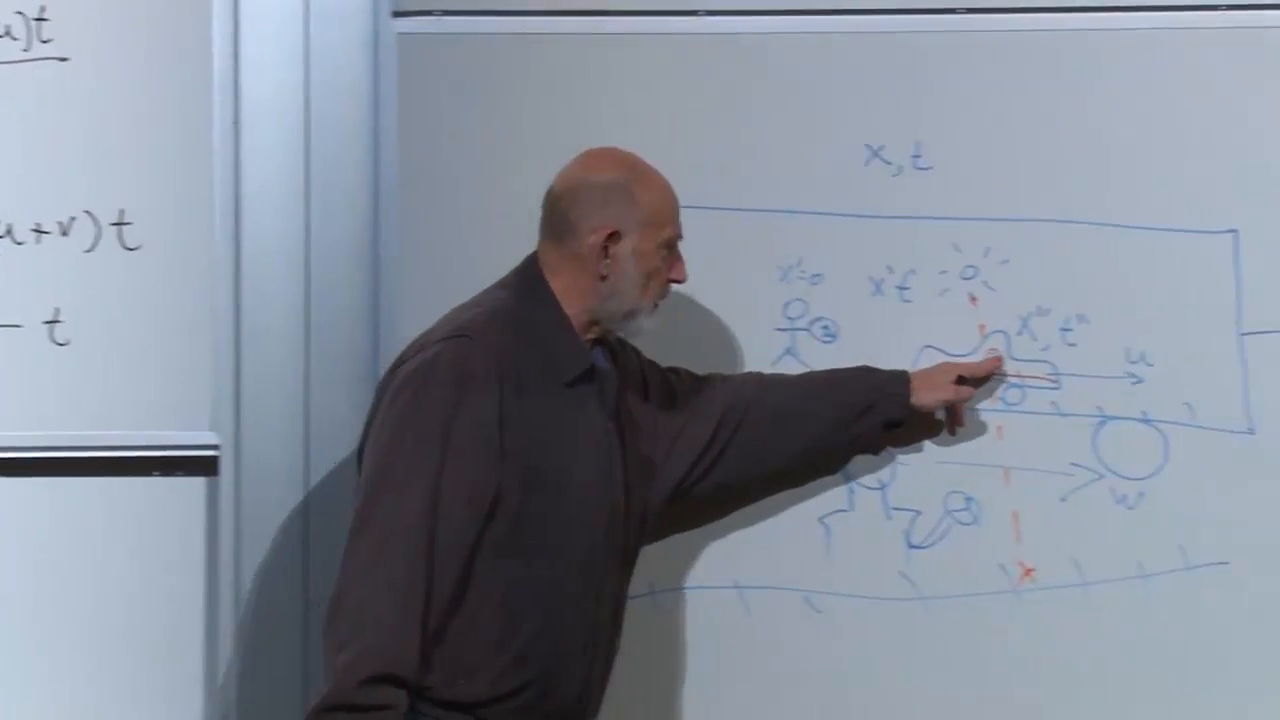
\includegraphics[width=0.91\textwidth]{lecture_02_figure_04.png}
\caption{La sustitución anidada antes de agrupar los términos en \(x\) y en \(t\) del impulso compuesto.}
\lectureframe{00:16:30}
\end{figure}

Como antes, el denominador no importa para localizar el origen móvil. El cochecito está en reposo en \(x''=0\), así que el corchete de \eqref{eq:sr2-composed-space} debe anularse:
\begin{equation}
(1+uv)x-(u+v)t=0.
\end{equation}
Por tanto, su línea de universo en el sistema de referencia de la estación es
\begin{equation}
x=\frac{u+v}{1+uv}\,t,
\end{equation}
y su velocidad es
\begin{equation}
\boxed{w=\frac{u+v}{1+uv}}.
\label{eq:sr2-velocity-add-c1}
\end{equation}

\begin{figure}[htbp]
\centering
\includegraphics[width=0.91\textwidth]{lecture_02_figure_05.png}
\caption{El numerador agrupado y la línea de universo \(x=[(u+v)/(1+uv)]t\) revelan la velocidad compuesta.}
\lectureframe{00:19:30}
\end{figure}

La ecuación temporal también se compone de manera consistente. La transformación completa de la estación al cochecito tiene la forma de Lorentz
\begin{align}
x''&=\gamma_w(x-wt),&
t''&=\gamma_w(t-wx),
\end{align}
donde
\begin{equation}
\gamma_w=\frac{1}{\sqrt{1-w^2}}.
\end{equation}
En efecto,
\begin{equation}
\gamma_w=\gamma_u\gamma_v(1+uv),
\end{equation}
lo cual se obtiene sustituyendo \eqref{eq:sr2-velocity-add-c1} y simplificando. Por tanto, dos impulsos colineales se componen en otro impulso colineal.

\subsection{Restitución de las dimensiones}

\begin{classroomqa}
\audiencequestion{¿Por qué el denominador \(1+uv\) es dimensionalmente incorrecto en unidades ordinarias?}
\lecturerresponse{Solo es correcto porque \(c=1\) hace que cada velocidad sea una fracción adimensional de la velocidad de la luz. En unidades convencionales, el producto debe aparecer como \(uv/c^2\), que es adimensional. \lecturetimestamp{00:21:11}}
\end{classroomqa}

La ley de adición de velocidades con dimensiones es
\begin{equation}
\boxed{
w=\frac{u+v}{1+\dfrac{uv}{c^2}}
}.
\label{eq:sr2-velocity-add}
\end{equation}

\begin{figure}[htbp]
\centering
\includegraphics[width=0.90\textwidth]{lecture_02_figure_06.png}
\caption{La consistencia dimensional restituye \(c^2\) debajo del producto \(uv\).}
\lectureframe{00:22:06}
\end{figure}

Para \(\lvert u\rvert,\lvert v\rvert\ll c\),
\begin{equation}
\frac{uv}{c^2}\ll 1,
\end{equation}
por lo que
\begin{equation}
w\approx u+v.
\end{equation}
La adición newtoniana es una aproximación válida a bajas velocidades, no una regla distinta.

\subsection{Dos regímenes numéricos}

Consideremos primero
\begin{equation}
u=v=0.01c.
\end{equation}
En unidades \(c=1\),
\begin{equation}
w=\frac{0.02}{1.0001}\approx 0.019998.
\end{equation}
El uno por ciento de la velocidad de la luz ya equivale aproximadamente a \(3\times10^6\ {\rm m/s}\), pero la corrección relativista es de solo una parte entre diez mil. El resultado es ligeramente menor que el valor newtoniano \(0.02c\).

\begin{figure}[htbp]
\centering
\includegraphics[width=0.90\textwidth]{lecture_02_figure_07.png}
\caption{Para \(u=v=0.01c\), el denominador difiere de uno en solo \(10^{-4}\).}
\lectureframe{00:24:23}
\end{figure}

Consideremos ahora
\begin{equation}
u=v=0.9c.
\end{equation}
Newton predeciría \(1.8c\). La relatividad da
\begin{equation}
\frac{w}{c}
=\frac{0.9+0.9}{1+0.9^2}
=\frac{1.8}{1.81}
\approx 0.9945.
\label{eq:sr2-fast-example}
\end{equation}

\begin{figure}[htbp]
\centering
\includegraphics[width=0.90\textwidth]{lecture_02_figure_08.png}
\caption{Dos velocidades de \(0.9c\) se componen en \(1.8/1.81\), todavía por debajo de la velocidad de la luz.}
\lectureframe{00:25:48}
\end{figure}

Una sucesión de impulsos sublumínicos no puede superar \(c\). Si \(u<c\) y \(v<c\), entonces
\begin{equation}
1-\frac{w}{c}
=
\frac{\left(1-\frac{u}{c}\right)
      \left(1-\frac{v}{c}\right)}
     {1+\frac{uv}{c^2}}
>0.
\end{equation}
Cada impulso adicional puede acercar el resultado a \(c\), pero nunca hacerlo superarlo. En el valor límite \(u=c\),
\begin{equation}
w=\frac{c+v}{1+v/c}=c.
\end{equation}
La velocidad de la luz es un punto fijo de la ley de composición.

\section{La medición de coordenadas no es la apariencia visual}

\begin{classroomqa}
\audiencequestion{Si el tren tuviera paredes de vidrio, ¿podría el observador de la estación mirar sin más al pasajero y al cochecito juntos y determinar directamente sus movimientos?}
\lecturerresponse{La transformación de Lorentz se refiere a mediciones de coordenadas realizadas con reglas distribuidas y relojes sincronizados. Una imagen visual también incluye los distintos tiempos que tarda la luz en llegar al observador desde sucesos diferentes. El vidrio cambia lo que se ve, no la relación entre las coordenadas; interpretar una sola imagen como datos simultáneos volvería a introducir precisamente el supuesto de simultaneidad que la relatividad corrigió. \lecturetimestamp{00:27:53}}
\end{classroomqa}

Un suceso tiene una posición y un tiempo en cada sistema de referencia, tanto si alguien lo ve en ese momento como si no. La apariencia óptica es un tema legítimo, pero requiere un segundo cálculo que siga la luz desde cada suceso hasta el ojo. Las leyes de transformación son universales e independientes de las paredes del tren.

\section{El intervalo propio en tres dimensiones espaciales}

Volvamos a dos sucesos: uno inicialmente en el origen y el otro en \((x,t)\). En una dimensión espacial,
\begin{equation}
\tau^2=t^2-x^2
\label{eq:sr2-interval-1d}
\end{equation}
en unidades \(c=1\). Todos los sistemas inerciales coinciden:
\begin{equation}
\tau^2
=t^2-x^2
=t'^2-x'^2
=t''^2-x''^2.
\end{equation}
Las coordenadas cambian; el intervalo propio no.

Para una separación temporal, un reloj puede desplazarse entre los sucesos. Si marca el mediodía en el primer suceso, la lectura transcurrida en el segundo es el tiempo propio \(\tau\). Esta afirmación es independiente del sistema de coordenadas que se use para calcular el intervalo.

\begin{figure}[htbp]
\centering
\includegraphics[width=0.90\textwidth]{lecture_02_figure_09.png}
\caption{Se recuerda la relación invariante para el tiempo propio \(\tau^2=t^2-x^2\) antes de restituir las direcciones transversales.}
\lectureframe{00:30:18}
\end{figure}

\subsection{Las rotaciones espaciales restituyen las direcciones transversales}

Consideremos una rotación ordinaria de los ejes espaciales antes de volver a los impulsos. Un punto que no esté sobre el eje \(x\) tiene una distancia espacial al cuadrado
\begin{equation}
r^2=x^2+y^2+z^2,
\end{equation}
que es invariante bajo rotaciones por el teorema de Pitágoras ordinario. En consecuencia, el intervalo del espacio-tiempo \(3+1\) es
\begin{equation}
\boxed{
\tau^2=t^2-x^2-y^2-z^2
}.
\label{eq:sr2-interval-3d}
\end{equation}
Al restituir \(c\),
\begin{equation}
c^2\tau^2
=c^2t^2-x^2-y^2-z^2.
\end{equation}

\begin{figure}[htbp]
\centering
\includegraphics[width=0.90\textwidth]{lecture_02_figure_10.png}
\caption{La distancia espacial pitagórica extiende el invariante de \(t^2-x^2\) a \(t^2-x^2-y^2-z^2\).}
\lectureframe{00:34:23}
\end{figure}

Cualquier combinación de rotaciones espaciales e impulsos de Lorentz preserva \eqref{eq:sr2-interval-3d}. Los ejes de coordenadas ordinarios discrepan sobre las componentes, pero coinciden en la distancia euclidiana; los sistemas inerciales del espacio-tiempo discrepan sobre las componentes espaciales y temporales, pero coinciden en esta diferencia de cuadrados. Este invariante es el hecho geométrico central de la relatividad especial.

\begin{classroomqa}
\audiencequestion{Si el pasajero sustituye el cochecito por un haz de luz dirigido hacia delante, ¿obtienen los observadores del tren y de la estación la misma velocidad de la luz?}
\lecturerresponse{Tomemos \(u=c\) en \eqref{eq:sr2-velocity-add}. Entonces \(w=(c+v)/(1+v/c)=c\). En unidades \(c=1\), el cociente es sencillamente \((1+v)/(1+v)=1\). Ambos sistemas de referencia miden la misma velocidad, exactamente como exige el postulado. \lecturetimestamp{00:35:53}}
\end{classroomqa}

Por tanto, la inquietud anterior sobre las paredes de vidrio no indica que falle la invariancia de la velocidad de la luz. Se trata de una confusión entre una medición de coordenadas y una imagen visual retardada; en último término, de una confusión sobre la simultaneidad.

\section{Rayos nulos y el cono de luz}

En una dimensión espacial, los rayos de luz que avanzan hacia la derecha o hacia la izquierda satisfacen
\begin{equation}
x=\pm t.
\end{equation}
Su intervalo se anula:
\begin{equation}
t^2-x^2=0.
\end{equation}
A diferencia de la distancia euclidiana, un intervalo espacio-temporal nulo no exige que los sucesos coincidan. Significa que una señal luminosa puede conectar uno con otro.

Al restituir todas las direcciones espaciales, un rayo de luz obedece
\begin{equation}
t^2-x^2-y^2-z^2=0,
\label{eq:sr2-null}
\end{equation}
o bien
\begin{equation}
r=t
\end{equation}
para la luz dirigida hacia el futuro en unidades \(c=1\).

\begin{figure}[htbp]
\centering
\includegraphics[width=0.90\textwidth]{lecture_02_figure_11.png}
\caption{La luz en cualquier dirección espacial sigue una trayectoria nula que satisface \(t^2-(x^2+y^2+z^2)=0\).}
\lectureframe{00:39:28}
\end{figure}

En \(1+1\) dimensiones, el conjunto nulo consiste en un par de rectas de \(45^\circ\). Con dos dimensiones espaciales más el tiempo, se convierte en un cono; las tres dimensiones espaciales no se pueden representar por completo en una pizarra, pero la ecuación que lo define no cambia.

El cono de luz futuro está formado por los sucesos a los que puede llegar la luz emitida en el origen. El cono de luz pasado está formado por los sucesos desde los que la luz puede llegar al origen. Uno es el otro invertido en el tiempo.

\begin{figure}[htbp]
\centering
\includegraphics[width=0.90\textwidth]{lecture_02_figure_12.png}
\caption{Los rayos nulos de \(45^\circ\) trazan los conos de luz futuro y pasado en un diagrama del espacio-tiempo de dimensión superior.}
\lectureframe{00:40:47}
\end{figure}

\begin{classroomqa}
\audiencequestion{¿Cuál es el invariante correspondiente bajo las transformaciones galileanas de la mecánica newtoniana?}
\lecturerresponse{El propio intervalo de tiempo. Todos los observadores newtonianos coinciden en \(\Delta t\), aunque discrepen sobre el desplazamiento espacial. La relatividad renuncia al tiempo universal y lo reemplaza por el intervalo espacio-temporal invariante. \lecturetimestamp{00:41:53}}
\end{classroomqa}

\section{De los vectores espaciales a los cuatro-vectores}

Los vectores de aquí son vectores geométricos, no vectores de estado cuánticos. Un desplazamiento entre dos puntos del espacio ordinario tiene módulo y dirección. Su origen puede trasladarse al origen de coordenadas sin que cambie el vector, y sus tres componentes pueden denotarse
\begin{equation}
x^i=(x^1,x^2,x^3)=(x,y,z),
\qquad i=1,2,3.
\end{equation}
El índice latino \(i\) recorre únicamente las direcciones espaciales.

Un suceso requiere una componente adicional: el tiempo. Por tanto, la posición en el espacio-tiempo se escribe
\begin{equation}
x^\mu=(x^0,x^1,x^2,x^3)=(t,x,y,z),
\qquad \mu=0,1,2,3.
\label{eq:sr2-four-position}
\end{equation}
Por convención histórica, el tiempo es la componente cero, no la cuarta:
\begin{equation}
x^0=t,\qquad x^1=x,\qquad x^2=y,\qquad x^3=z.
\end{equation}
Los índices griegos, como \(\mu\), recorren el espacio-tiempo; los índices latinos, como \(i\), recorren el espacio.

\begin{figure}[htbp]
\centering
\includegraphics[width=0.90\textwidth]{lecture_02_figure_13.png}
\caption{Las componentes espaciales \(x^i\) se amplían a la posición espacio-temporal de cuatro componentes \(x^\mu=(x^0,x^1,x^2,x^3)\).}
\lectureframe{00:46:05}
\end{figure}

El invariante se convierte en
\begin{equation}
\tau^2
=(x^0)^2-(x^1)^2-(x^2)^2-(x^3)^2.
\end{equation}
La notación por sí sola no añade nueva física. Su utilidad consiste en que una transformación de Lorentz actúa linealmente sobre las cuatro componentes, del mismo modo que una rotación actúa linealmente sobre un vector espacial.

\begin{classroomqa}
\audiencequestion{Dado que la transformación es lineal, ¿se puede representar mediante una matriz que actúe sobre un vector columna?}
\lecturerresponse{Sí. Para un impulso a lo largo de \(x\), el bloque no trivial es \(\gamma_v\begin{pmatrix}1&-v\\-v&1\end{pmatrix}\), que actúa sobre \((t,x)^{\mathsf T}\), mientras que \(y\) y \(z\) no cambian. La notación matricial es la manera natural de componer y organizar las transformaciones de Lorentz. \lecturetimestamp{00:48:14}}
\end{classroomqa}

Explícitamente,
\begin{equation}
\begin{pmatrix}
t'\\x'\\y'\\z'
\end{pmatrix}
=
\begin{pmatrix}
\gamma_v&-\gamma_v v&0&0\\
-\gamma_v v&\gamma_v&0&0\\
0&0&1&0\\
0&0&0&1
\end{pmatrix}
\begin{pmatrix}
t\\x\\y\\z
\end{pmatrix}.
\label{eq:sr2-boost-matrix}
\end{equation}

\section{Desplazamientos y cuadrivelocidad}

Pasemos de la posición de un suceso a un segmento corto de la línea de universo de una partícula. El cuadridesplazamiento es
\begin{equation}
\Delta x^\mu
=(\Delta t,\Delta x,\Delta y,\Delta z).
\end{equation}
Al llamar pequeño a un desplazamiento, nos acercamos al cálculo diferencial: \(\Delta x^\mu\) se convertirá en \(dx^\mu\). Por ahora, la notación finita hace transparente la geometría.

El incremento de tiempo propio a lo largo de una línea de universo temporal satisface
\begin{equation}
(\Delta\tau)^2
=(\Delta t)^2-(\Delta x)^2-(\Delta y)^2-(\Delta z)^2.
\label{eq:sr2-proper-increment}
\end{equation}
La velocidad ordinaria divide el desplazamiento espacial por el tiempo coordenado y tiene tres componentes. En cambio, la cuadrivelocidad divide el cuadridesplazamiento por el tiempo propio invariante:
\begin{equation}
u^\mu
=\frac{\Delta x^\mu}{\Delta\tau}
\quad\longrightarrow\quad
\boxed{
u^\mu=\frac{dx^\mu}{d\tau}
}.
\label{eq:sr2-four-velocity}
\end{equation}

\begin{figure}[htbp]
\centering
\includegraphics[width=0.90\textwidth]{lecture_02_figure_14.png}
\caption{Un segmento de línea de universo define \(\Delta x^\mu\), su invariante \(\Delta\tau\) y la cuadrivelocidad \(u^\mu=\Delta x^\mu/\Delta\tau\).}
\lectureframe{00:52:42}
\end{figure}

Este objeto tiene cuatro componentes y se transforma como un cuatro-vector. La relación entre esta cantidad y la velocidad tridimensional ordinaria es la siguiente pregunta, que aquí se deja deliberadamente abierta. Resolverla nos conduce hacia el momento relativista, la energía, la aceleración y, en último término, la generalización relativista de \(F=ma\).